%%%%%%%%%%%%%%%%%%%%%%%%%%%%%%%%%%%%%%%%%%%%%%%%%%%%%%%%%%%%%%%%%%%%%%%%%%%%%%%%%
%% Document: Thesis for PhD at UC Riverside                                    %%
%% Title: Investigating the evolution of environmental and biotic interactions %%
%%          in basal fungal lineages through comparative genomics              %%
%% Author: Steven Ahrendt                                                      %%
%%%%%%%%%%%%%%%%%%%%%%%%%%%%%%%%%%%%%%%%%%%%%%%%%%%%%%%%%%%%%%%%%%%%%%%%%%%%%%%%%
%% APPENDIX FIGURES %%
%%%%%%%%%%%%%%%%%%%%%%

% Flagellar heat map from James et al 2009
\begin{figure}
  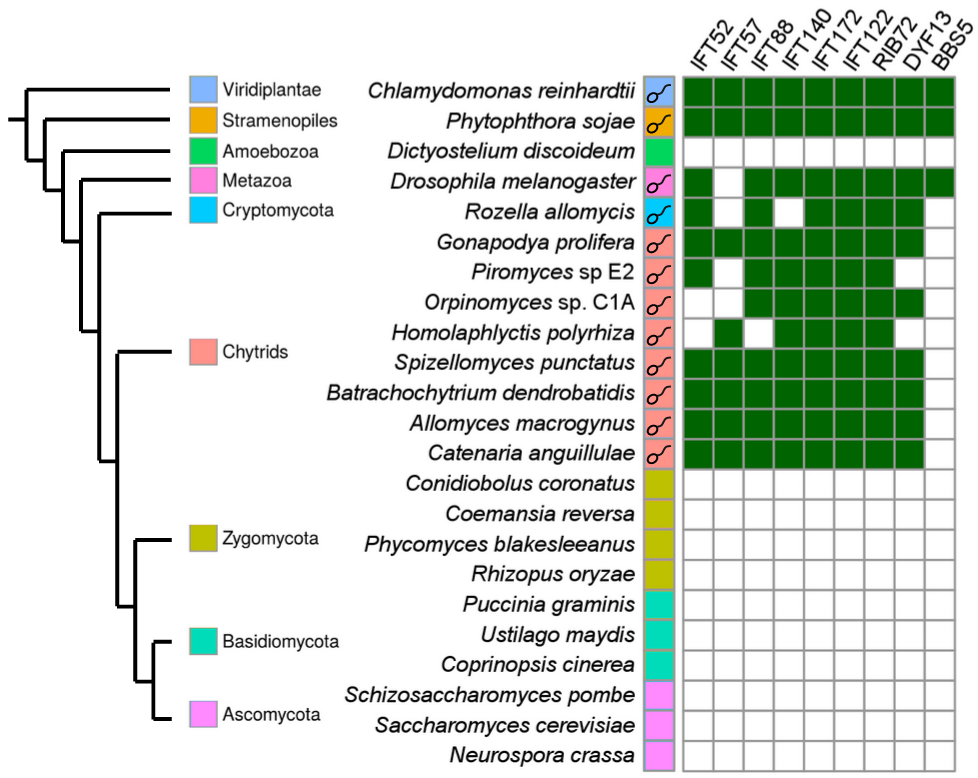
\includegraphics[width=4in]{./Appendix/img/flagDataHeatmap_subset.png}
  \caption[Heatmap cluster analysis of flagellar proteins from \textit{Naegleria gruberi}]{A subset of proteins which cluster according to presence/absence in flagellated and non-flagellated organisms. Protein copies identified in proteomes of interest are normalized to indicate presence and absence only, where green indicates that one or more copies were found.}
  \label{fig:AppFlag_heatmap}
\end{figure}
